\documentclass[11pt,letterpaper]{article}
\usepackage[lmargin=1in,rmargin=1in,tmargin=1in,bmargin=1in]{geometry}
\usepackage{../style/homework}
\setbool{quotetype}{true} % True: Side; False: Under
\setbool{hideans}{false} % Student: True; Instructor: False

\newcommand{\squiggle}{\rightsquigarrow}

% -------------------
% Content
% -------------------
\begin{document}

\homework{11: Due 03/06}{The universe is basically an animal. It grazes on the ordinary. It creates infinite idiots just to eat them.}{Rick Sanchez, Rick and Morty}

% Problem 1
\problem{10} Suppose that the number of people served at the DMV is uniformly distributed over the 8 hours that they are open (9~am to 5~pm). 
	\begin{enumerate}[(a)]
	\item What percentage of people are served before noon?
	\item What percentage of people are served after noon?
	\item What percentage of people are served between 11~am and 3~pm? 
	\item At what time has the DMV served 90\% of the people they will assist that day?
	\end{enumerate} \pspace

\sol We can draw a sketch of this scenario:
	\[
	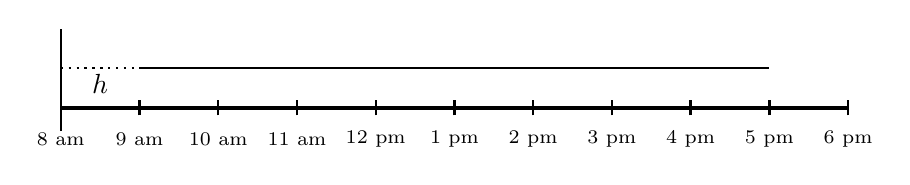
\begin{tikzpicture}
	\draw[line width=0.05cm] (0,0) -- (10,0);
						
	\foreach \i [evaluate=\i as \x using \i - 8] in {8,9,...,11} {
	\draw[line width=0.03cm] (\x,-0.1) -- (\x,0.1);
	\node at (\x,-0.4) {\scriptsize \i~am};
						};
	\foreach \i [evaluate=\i as \x using \i + 4] in {1,2,...,6} {
	\draw[line width=0.03cm] (\x,-0.1) -- (\x,0.1);
	\node at (\x,-0.4) {\scriptsize \i~pm};
						};
	
	\draw[line width=0.03cm] (4,-0.1) -- (4,0.1);
	\node at (4,-0.4) {\scriptsize 12~pm};
	
	\draw[line width=0.03cm] (1,0.5) -- (9,0.5);
	
	\draw[line width=0.03cm] (0,-0.3) -- (0,1);
	\draw[line width=0.03cm,dotted] (0,0.5) -- (1,0.5);
	\node at (0.5,0.3) {$h$};
	\end{tikzpicture}
	\]
We want to choose the height $h$ so the area under the uniform distribution is 1. But this area is a rectangle. We know $A= \ell h$. So $1= 8h$, which implies $h= \frac{1}{8}$.

\begin{enumerate}[(a)]
\item This is the area under the curve before noon:
	\[
	P(t \leq 12)= 3 \cdot \dfrac{1}{8}= \dfrac{3}{8} \approx 0.375
	\] \pspace

\item 
	\[
	P(t \geq 12)= 1 - P(\leq 12)= 1 - \dfrac{3}{8}= \dfrac{5}{8} \approx 0.625
	\] \pspace

\item 
	\[
	P(11 \leq t \leq 3)= 4 \cdot \dfrac{1}{8}= \dfrac{4}{8}= \dfrac{1}{2} \approx 0.50
	\] \pspace

\item We want a time, $T$, such that $P(t \leq T)= 0.90$. But then\dots
	\[
	0.90= P(t \leq T)= T \cdot \dfrac{1}{8}= \dfrac{T}{8}
	\]
This implies that $T= 7.2$, i.e. 7.2~hours after opening. We know 0.20~hours is $60 \cdot 0.20= 12$~minutes. Seven hours after 8~am is 3~pm. But then the DMV has served 90\% of people by 3:12~pm.
\end{enumerate}





\newpage



% Problem 2
\problem{10} Suppose you have a normal distribution with mean $\mu= 870$ and standard deviation $\sigma= 113$. Showing all your work, compute the following:
	\begin{enumerate}[(a)]
	\item $P(X= 900)$
	\item $P(X < 950)$
	\item $P(X > 950)$
	\item $P(800 < X < 950)$
	\end{enumerate} \pspace

\sol 
\begin{enumerate}[(a)]
\item In a continuous distribution, e.g. the normal distribution, $P(X= \#)= 0$. Therefore, we have\dots
	\[
	P(X= 900)= 0 
	\] \pspace

\item We have\dots
	\[
	z_{950}= \dfrac{950 - 870}{113}= \dfrac{80}{113} \approx 0.71 \squiggle 0.7611
	\]
Therefore, $P(X < 950)= 0.7611$. \pspace

\item We have\dots
	\[
	P(X > 950)= 1 - P(X < 950)= 1 - 0.7611= 0.2389
	\] \pspace

\item We have\dots
	\[
	z_{800}= \dfrac{800 - 870}{113}= \dfrac{-70}{113}= -0.62 \squiggle 0.2676
	\]
But then\dots
	\[
	P(800 < X < 950)= P(X < 950) - P(X < 800)= 0.7611 - 0.2676= 0.4935
	\]
\end{enumerate}


\end{document}